\chapter{GOAP Umsetzung in Godot}

Die praktische Umsetzung des GOAP Systems wird nun in diesem Kapitel beschrieben. Die Umsetzung passiert auf Basis der Publikation von Jeff Orkin. Die Implementierung geschieht unter der Godot Engine 4.3. Das Kapitel wird zuerst die grundlegende Architektur von GOAP anhand eines Agenten beschreiben.[Kapitel weiter erläutern]

\section{GOAP Architektur}

Die folgende Abbildung soll die grundlegende Architektur von GOAP darstellen. Die Darstellung wird anhand eines Klassendiagramms in UML-Notation umgesetzt.

\begin{figure}[h]
  \centering
  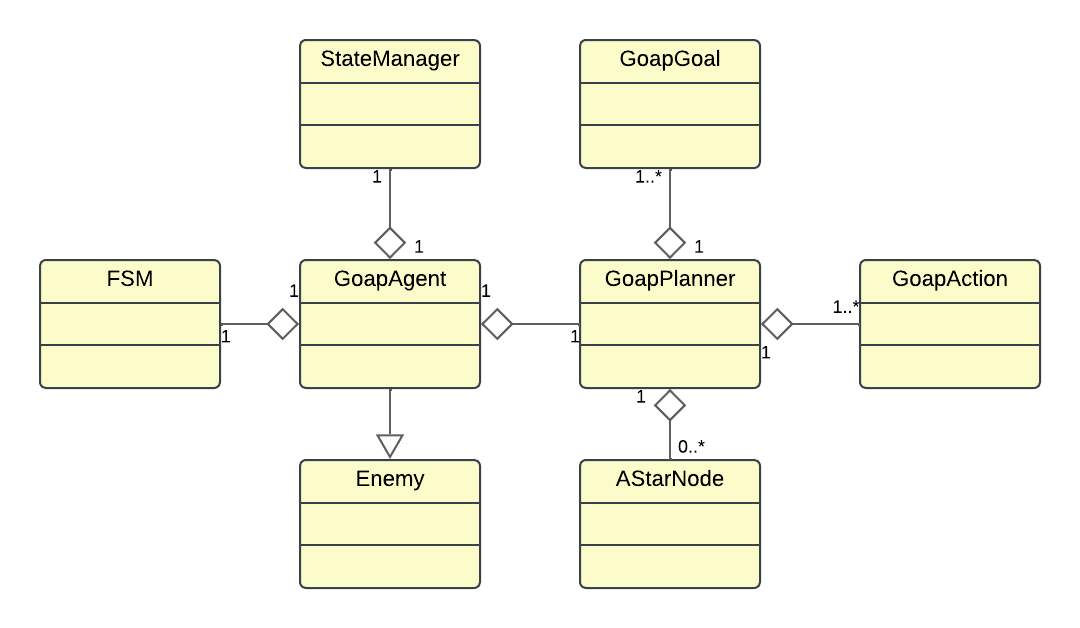
\includegraphics[width=16cm]{GOAP_2/GOAP_UML}
	\captionsetup{justification=justified, format=plain}
  \caption{GOAP Architektur}
  \label{GOAP Architektur eines Agenten}
\end{figure}

Aus dem GOAP-Kapitel geht hervor, dass ein GOAP-System aus einem Planner, Zielen, Aktionen und einer FSM (Finite State Machine) besteht. Diese Komponenten erfüllen ihre jeweiligen Aufgaben, wie im Grundlagenkapitel über GOAP beschrieben.

Der GoapAgent bildet dabei die Hauptklasse und soll die Schnittstelle zur restlichen Spielwelt sein. Die Spielwelt kann ihm Informationen wie die Position des Spielers oder bestimmte Koordinaten innerhalb der Spielwelt übermitteln. Dabei erbt der GoapAgent von der Klasse Enemy. Die Klasse Enemy stellt Komponenten bereit, die es dem GoapAgent ermöglichen, mit der Spielwelt zu interagieren.

Der StateManager verwaltet die Zustände des NPC. Diese Zustände können über die Komponenten der Oberklasse Enemy verändert werden können.

Die FSM setzt die Aktionssequenz aus, welche im GoapAgent gespeichert wird. Sie kann neue Sequenzen an den Goap gent anfordern.

Zur Generierung von Sequenzen und Festlegung des Zieles benutzt der GoapAgent die Klasse GoapPlanner. Der GoapPlanner besitzt dabei Objekte der Klasse GoapGoal. Aus diesen Objekten entscheidet sich der GoapPlanner für ein Zielzustand, zu welchem eine Aktionssequenz gesucht wird.
Der GoapPlanner sucht seine Sequenz mithilfe des A* Suchalgorithmus. Die Klasse AStarNode wird zur Erstellung von Knoten für den A* Suchalgorithmus benötigt. Ein AStarNode setzt dabei die Eigenschaften eines Suchbaum-Knoten um [siehe Kapitel Suchproblem, Knoten].

Die Klasse GoapAction definiert die Basisklasse für Aktionen. Eine Aktion repräsentiert dabei eine Kante im Suchbaum und wird entsprechend als solche im AStarNode-Objekt gespeichert.

\subsection{GoapAgent}

GoapAgent

\begin{figure}[h]
  \centering
  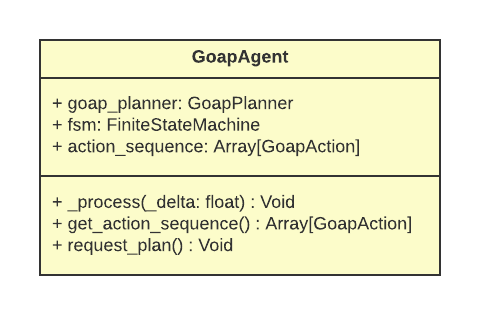
\includegraphics[width=10cm]{GOAP_2/GoapAgent_UML}
	\captionsetup{justification=justified, format=plain}
  \caption{GOAP Agent}
  \label{GOAP Agent}
\end{figure}